\documentclass[twocolumn,twoside]{article}

% Modified Template by Jonathan Doucette and Kevin Multani, original by: Jonathan Ward

\documentclass[12pt]{article} 
\usepackage[english]{babel}
\usepackage[utf8]{inputenc}
\usepackage{amsmath} % AMS Math Package
\usepackage{amsthm} % Theorem Formatting
\usepackage{amssymb} % Math symbols such as \mathbb
\usepackage{graphicx} % Allows for eps images
\usepackage{multicol} % Allows for multiple columns
\usepackage[dvips,letterpaper,margin=1in,bottom=1in]{geometry}
\usepackage{hyperref}
\usepackage{parskip} % Removes indentation from paragraphs
\usepackage{xcolor,xspace,soul} % Colour, spacing, and highlighting
\usepackage{mathrsfs}
\usepackage{bm} % For bold math symbols
\usepackage{amscd}
\usepackage[all,cmtip]{xy}
%\usepackage{bbm}
\usepackage{titling}
\usepackage{listing} % for code snippets
%\usepackage{minted} % for code snippets
\usepackage{enumerate}
\usepackage{fancyhdr}
\usepackage[]{physics}
\usepackage[makeroom]{cancel}
\usepackage{pdfpages}
\usepackage[]{mcode}
\usepackage[title]{appendix}

% ***********************************************************
% ********************** BEGIN TITLE PAGE *******************
% ***********************************************************
\newcommand*{\titleGM}{\begingroup % Create the command for including the title page in the document
\hbox{ % Horizontal box
\hspace*{0.2\textwidth} % Whitespace to the left of the title page
\rule{1pt}{\textheight} % Vertical line
\hspace*{0.05\textwidth} % Whitespace between the vertical line and title page text
\parbox[b]{0.75\textwidth}{ % Paragraph box which restricts text to less than the width of the page

{\noindent\Huge\bfseries MATH 521}\\[2\baselineskip] % Title
{\large \textit{Assignment 4}}\\[4\baselineskip]
%{\large \textsc{ Jonathan Doucette }} % Author name

\vspace{0.5\textheight} % Whitespace between the title block and the publisher
{\noindent \today }\\[\baselineskip]
%{\noindent Student Number: 35298124 }\\[\baselineskip] 
%{\noindent \footnotesize All problems below are \textit{Copyright \copyright \space 2018 Timm Treskatis. All Rights Reserved.} }\\[\baselineskip]
} % end parbox
} % end hbox
\endgroup}

 % Sets margins and page size
\pagestyle{fancy} 

%\lhead{Jonathan Doucette}
\rhead{\today}
\rfoot{Page \thepage}
\cfoot{}

\makeatletter % Need for anything that contains an @ command 
\renewcommand{\maketitle} % Redefine maketitle to conserve space
{ \begingroup \vskip 10pt \begin{center} \Huge {\bf \@title}
\vskip 10pt \large \@author \hskip 20pt \@date \end{center}
  \vskip 10pt \endgroup \setcounter{footnote}{0} }
\makeatother % End of region containing @ commands

% ***********************************************************
% ********************** END TITLE PAGE *********************
% ***********************************************************

% ***********************************************************
% ********************** BEGIN NEW COMMANDS *****************
% ***********************************************************

\renewcommand{\labelenumi}{(\alph{enumi})} % Use letters for enumerate
\let\vaccent=\v % rename builtin command \v{} to \vaccent{}

%% MISC
\newcommand{\ab}[1]{\left| #1 \right|} % for absolute value
\newcommand{\avg}[1]{\left< #1 \right>} % for average
\let\underdot=\d % rename builtin command \d{} to \underdot{}
\let\baraccent=\= % rename builtin command \= to \baraccent
\renewcommand{\=}[1]{\stackrel{#1}{=}} % for putting numbers above =
\providecommand{\fr}{\frac}
\providecommand{\RR}{\mathbb{R}}
\providecommand{\CC}{\mathbb{C}}
\providecommand{\NN}{\mathbb{N}}
\providecommand{\e}{\epsilon}
\DeclareMathOperator{\di}{d\!}
\newcommand*\ieval[3]{\left.#1\right\rvert_{#2}^{#3}}

%% Vectors
\renewcommand{\v}[1]{\ensuremath{\mathbf{#1}}} 
\newcommand{\gv}[1]{\ensuremath{\mbox{\boldmath$ #1 $}}} % for vectors of Greek letters
\newcommand{\uv}[1]{\ensuremath{\mathbf{\hat{#1}}}} % for unit vector
\providecommand{\wave}[1]{\v{\tilde{#1}}}

%% DERIVATIVES
\renewcommand{\d}[2]{\frac{d #1}{d #2}} % for derivatives
\newcommand{\dubd}[2]{\frac{d^2 #1}{d #2^2}} % for double derivatives
\newcommand{\pd}[2]{\frac{\partial #1}{\partial #2}} % for partial derivatives
\newcommand{\pdd}[2]{\frac{\partial^2 #1}{\partial #2^2}} % for double partial derivatives

%% Operators
\newcommand{\Gradient}{\ensuremath{\mbox{\boldmath$\nabla$}}} % gradient

%% Text
\newcommand{\mathcolorbox}[2]{\colorbox{#1}{$\displaystyle #2$}}
\newcommand{\hlfancy}[3]{\textcolor{#1}{\sethlcolor{#2}\hl{#3}}}
\newcommand{\TODO}[1]{\hlfancy{red}{yellow}{\textbf{TODO: #1}}}

%% Code
%\newcommand{\code}[1]{\mintinline{C}{#1}}
%\newcommand{\code}[1]{\texttt{#1}}
\newcommand{\code}[1]{\lstinline[columns=fixed]{#1}}
\newcommand{\includecode}[1]{\lstinputlisting{#1}}

% ***********************************************************
% ********************** END NEW COMMANDS *******************
% ***********************************************************

% ***********************************************************
% ********************** BEGIN NEW ENVS *********************
% ***********************************************************

% Theorem
\newenvironment{theorem}[2][Theorem]{\begin{trivlist}
\item[\hskip \labelsep {\bfseries #1}\hskip \labelsep {\bfseries #2.}]}{\end{trivlist}}
% Lemma
\newenvironment{lemma}[2][Lemma]{\begin{trivlist}
\item[\hskip \labelsep {\bfseries #1}\hskip \labelsep {\bfseries #2.}]}{\end{trivlist}}
% Corollary
\newenvironment{corollary}[2][Corollary]{\begin{trivlist}
\item[\hskip \labelsep {\bfseries #1}\hskip \labelsep {\bfseries #2.}]}{\end{trivlist}}

% Exercise
\newenvironment{exercise}[2][Exercise]{\begin{trivlist}
\item[\hskip \labelsep {\bfseries #1}\hskip \labelsep {\bfseries #2.}]}{\end{trivlist}}
% Problem
\newenvironment{problem}[2][Problem]{\begin{trivlist}
\item[\hskip \labelsep {\bfseries #1}\hskip \labelsep {\bfseries #2.}]}{\end{trivlist}}
% Question
\newenvironment{question}[2][Question]{\begin{trivlist}
\item[\hskip \labelsep {\bfseries #1}\hskip \labelsep {\bfseries #2.}]}{\end{trivlist}}
% Solution
\newenvironment{solution}{\begin{proof}[Solution]}{\end{proof}}

% Afterword
\newenvironment{afterword}[2][Appendix]{\begin{trivlist}
\item[\hskip \labelsep {\bfseries #1}\hskip \labelsep {\bfseries #2}]}{\end{trivlist}}

% ***********************************************************
% ********************** END NEW ENVS ***********************
% ***********************************************************

% ***********************************************************
% ********************** END TITLEPAGE **********************
% ***********************************************************

%% ------------------------------------------------------ %%
%% ----------------------- Title ------------------------ %%
%% ------------------------------------------------------ %%

\setlength{\droptitle}{-0.5cm}
\title{Numerical Methods in Magnetic Resonance Imaging:\\The Bloch-Torrey Equation\vspace{0.3cm}}

\author[a,b]{Jonathan Doucette}

\affil[a]{UBC MRI Research Centre, University of British Columbia,
  2221 Wesbrook Mall, Vancouver, BC, Canada.}

\affil[b]{Department of Physics and Astronomy, University of British
  Columbia, 6224 Agricultural Road, Vancouver, BC, Canada.\vspace{0.3cm}}

\date{\today}
\setcounter{Maxaffil}{0}
\renewcommand\Affilfont{\itshape\small}

\begin{document}

\maketitle

%Corresponding author footer
\let\thefootnote\relax\footnote{e-mail: \texttt{jdoucette@phas.ubc.ca}}
%{\let\thefootnote\relax\footnote{{\textsuperscript{†}e-mail: jdoucette@phas.ubc.ca}}}

%TODO Abstract
\vspace{-0.63cm}
\TODO{final spacing}
\textbf{In magnetic resonance imaging, insight into different imaging modalities can be gained through the simulation of the magnetic resonance signal measured by the scanner.
This signal is modelled as the solution of the parabolic Bloch-Torrey partial differential equation.
In this work, I compare various numerical techniques for solving the Bloch-Torrey equation in the presence of highly discontinuous data with the goal of optimising the trade-off between solution accuracy and computation time.}

\section*{Introduction}
In magnetic resonance imaging (MRI), insight into different imaging modalities can be gained through the simulation of the magnetic resonance (MR) signal from first principles.
The MR signal which is measured by an MRI scanner within a given region  is directly proportional to the magnitude of the net magnetization vector \MM{} within that region.
In tissue, \MM{} arises due to the superposition of the magnetic moments of water molecules, also known as \textit{spins} in MRI nomenclature.
Ordinarily, \MM{} is zero in tissue as spins are randomly oriented and therefore their vector sum is zero on the average.
In MRI, however, there is a large and constant external magnetic field $\v{B_0} = B_0 \uv{z}$ which forces the alignment of the magnetized spins with $\v{B_0}$, taken here to be along the $z$-direction.
This allows for the measurement, and importantly, the manipulation of the otherwise negligible net magnetization \MM{} of the spins.

In one common type of MRI scan, a \textit{gradient echo} scan, \MM{} is initially flipped into the $xy$-plane through the application of a radio frequency (RF) magnetic pulse.
Immediately, \MM{} begins to realign with $\v{B_0}$ exponentially quickly.
The rate \rr{} at which this realignment occurs, however, depends on local tissue properties. % and therefore the realignment occurs at different rates at different locations in space.
Additionally, there is a characteristic precession of \MM{} about $\v{B_0}$ as it realigns.
This precession occurs at a rate \ww{} which, too, depends on the magnetic properties of the environment.
Lastly, spins are free to diffuse within their environment while realigning, which means that they will see varying \rr{} and \ww{} as they move through the tissue.

\subsection*{The Bloch-Torrey equation}

In the continuum limit, the net magnetization \MM{} within a given region is modelled as a continuous vector field, and the complex dynamics which follow the initial RF pulse can be beautifully modelled as solutions to a parabolic partial differential equation (PDE) called the Bloch-Torrey equation~\cite{torrey_bloch_1956}:
%
\begin{equation}\label{BTreal}
\begin{cases}
\ddt{u} = D \Laplacian{u} - R u + \omega v\\%, \qquad u(\v{x},0) = M_x(\v{x},0) \\
\hspace{0.8pt}\ddt{v} = D \Laplacian{v} - R v - \omega u\\%, \qquad \hspace{1pt} v(\v{x},0) = M_y(\v{x},0).
\end{cases}
\end{equation}
%
Here, $u$ and $v$ are the $x$- and $y$-components of the magnetization \MM{} and $D$ is the diffusion constant.
For short simulation times, or \textit{echo times}, $T$, the $z$-component of \MM{} does not change appreciably, and we need only consider the transverse magnetization $\Mt{} = (u,v)$.

The transverse Bloch-Torrey equation~\eqref{BTreal} may be equivalently written as
%
\begin{equation}\label{BTcplx}
\ddt{\Mxy} = D \Laplacian{\Mxy} - \CDecay \Mxy
\end{equation}
%
where $\Mxy = u + i v$ is the complex magnetization and $\CDecay(\v{x}) = R(\v{x}) + i \omega(\v{x})$ is the complex decay rate.
This form is both notationally convenient and conceptually illustrative; now, realignment with \Bo{} corresponds to the magnitude of the (complex) transverse magnetization $\Mxy$ decaying to zero, and the precession of \MM{} about \Bo{} corresponds to the rotation of $\Mxy$ about the origin in the complex plane.

\subsection*{Signal simulation}
This work will compare three different methods of simulating the signal $S(T)$ measured by an MRI scanner at a time $T$ following an initial RF pulse: finite differences, splitting methods, and finite element methods.

The MR signal $S(T)$ is given by
%
\begin{equation}
S(T) = \Norm{\int_\Omega \Mt{}(T) \dx{x}}
\end{equation}
%
where $\Mt{}(T)$ is computed by solving~\eqref{BTreal} or~\eqref{BTcplx}. The initial transverse magnetization $\Mt{}(t=0)$ will be taken to be $[0,1]^T$ without loss of generality.%, noting that multiplying~\eqref{BTcplx} by a complex constant $\alpha$ simply results in a final signal which is scaled by $\ab{\alpha}$.

\subsection*{Geometry}
The transverse magnetization $\Mt{}$ will be simulated within a cubic domain $\Omega$ of size $3\times3\times\SI{3}{mm^3}$ with a single cylinder of a variable radius $a$ in the centre of the domain, as pictured in Figure~\ref{fig:geometry}.

This geometry is chosen for two reasons.
First, biologically it represents a single vessel present within a cubic imaging voxel.
Second, there exists an exact solution for \ww{} given the magnetic susceptibility $\chi$ of the cylindrical blood vessel~\cite{cheng_limitations_2009}.
For a cylinder of radius $a$, we have that
%
\begin{equation}\label{omega}
\ww{} = 
\begin{cases}
\frac{\chi B_0}{2}\sin^2\theta \frac{a^2}{x^2+y^2} \frac{y^2-x^2}{x^2+y^2}, \hspace{0.17cm} \text{outside cylinder}\\
\frac{\chi B_0}{6} \left(3\cos^2\theta - 1\right), \qquad \text{inside cylinder}
\end{cases}
\end{equation}
%
where $\theta$ is the angle between the cylinder axis and \Bo{}.
An example cross section of \ww{} can be seen in Figure~\ref{fig:geometry}.
Note that $\ww{}$ is constant within the cylinder, and jumps discontinuously to a smooth solution outside of the cylinder.

The transverse relaxation rate \rr{} is taken to be piecewise constant values inside and outside of the cylinder,
\begin{equation}\label{r2decay}
\rr{} = 
\begin{cases}
R_{\text{tissue}}, \quad \text{outside cylinder} \\
R_{\text{blood}}, \quad\hspace{0.02cm} \text{inside cylinder.}
\end{cases}
\end{equation}
where $0 < R_{\text{tissue}} < R_{\text{blood}}$ are positive constants.
%Both \ww{} and \rr{} are piecewise smooth with sharp discontinuities at the cylinder boundary.

\section*{Properties of the Bloch-Torrey equation}
%Finite difference methods, splitting methods, and finite element methods will be investigated.
%First, some basic properties of the Bloch-Torrey equation are described.

\subsection*{Static solution}

If $D = 0$, solutions to~\eqref{BTcplx} are simply complex exponentials
\begin{equation}\label{BTstatic_cplx}
\Mxy(\v{x},t) = \Mxy_0 e^{-\CDecay(\v{x}) t} \\
= \left(e^{-\rr{} t} \ab{\Mxy_0}\right) e^{i(\phi_0 - \ww{} t)},
\end{equation}
where we have written $\Mxy_0 = \ab{\Mxy_0} e^{i\phi_0}$ in polar form.
Equivalently, the static solution may be written
\begin{equation}\label{BTstatic_real}
\Mt{} = e^{-\rr{} t} \Norm{\Mt{}_0} \begin{pmatrix} \cos(\phi_0 - \ww{}t) \\ \sin(\phi_0 - \ww{}t) \end{pmatrix}.
\end{equation}
In this form, it is clear to see that the magnitude $\ab{\Mxy} = \Norm{\Mt{}}$ of the transverse magnetization is exponentially damped at rate \rr{} and that the initial phase $\phi_0$ changes at the constant rate \ww{}, which can be interpreted as the transverse magnetization rotating about \Bo{} at a constant angular velocity at each point in space.

\subsection*{Relation to the heat equation}
If $\CDecay = 0$, then~\eqref{BTreal} reduces to two uncoupled heat equations in the transverse magnetization components $u$ and $v$.
This is equivalent to the limit as the magnetic field $B_0 \rightarrow 0$, as the magnetic moments of the spins are not forced to realign with an external field and instead are free to diffuse unhindered.

Mathematically, we should expect that solutions to the Bloch-Torrey equation exhibit some of the same properties as solutions of the heat equation, such as exponential suppression of high frequency eigenmodes.

\subsection*{Relation to the reaction-diffusion equation}
The two-component reaction-diffusion equation, which models for example how the concentrations $u$ and $v$ of two chemicals change over time within a medium, is given by
\begin{equation}\label{RxnDiff}
\begin{cases}
\ddt{u} = D \Laplacian{u} + F(u,v)\\
\hspace{0.8pt}\ddt{v} = D \Laplacian{v} + G(u,v)\\
\end{cases}
\end{equation}
where $F$ and $G$ govern local chemical reactions which may increase or decrease the concentrations $u$ and $v$ depending on whether they are being produced or consumed.

The reaction-diffusion equation~\eqref{RxnDiff} corresponds directly to the Bloch-Torrey equation in the case of linear reaction terms $F = - R u + \omega v$ and $G = - R v - \omega u$.
In this interpretation, \rr{} represents the local rate at which $u$ and $v$ are reacted away into waste products, and \ww{} represents the local rate at which $u$ reacts into $v$ and vice versa. 
\TODO{double check this interpretation}

\subsection*{Weak form}
The coupled system of PDEs~\eqref{BTreal} can be written as
\begin{align}\label{BTvec}
\begin{cases}
\ddt{\uu{}} = -A \uu{} \quad\text{ in }\Omega,\quad t>0 \\
\hspace{3.5pt}\uu{} = \v{g} \qquad\hspace{6pt} \text{ in }\Omega,\quad t=0
\end{cases}
\end{align}
where $\uu{} = [u,v]^T$ and
\begin{align}
    A = \begin{pmatrix}
    -D \Laplacian{} + R & -\omega \\ 
    \omega & -D \Laplacian{} + R
    \end{pmatrix}.
\end{align}

Now, consider the vector test function $\v{v} = [w,z]^T$ where $w,z \in V = H^1$.
Then, the weak form of~\eqref{BTvec} is given by
\begin{align}\label{BTweak}
\langle \v{v}, \ddt{\uu{}} \rangle
&= - \langle \v{v}, A \uu{} \rangle, \quad \forall \v{v} \in V\!\times V
\end{align}
where
\begin{align*}
\langle \v{v}, A \uu{} \rangle
= \int_\Omega &\left\{-D w \Laplacian{u} + R w u - \omega w v \right. \\
&\left. -D z \Laplacian{v} + R z v + \omega z u \right\} \, \dx{x}.
\end{align*}
Applying zero Neumann boundary conditions on the boundary $\partial\Omega$, this simplifies to
\begin{align}\label{Abilinear}
\langle \v{v}, A \uu{} \rangle
= \int_\Omega & D \left(\Gradient{w}\cdot\Gradient{u} + \Gradient{z}\cdot\Gradient{v}\right) + \\
&R(w u + z v) + \omega (z u - w v) \, \dx{x}. \nonumber
\end{align}

\subsection*{Coercivity and local magnetization decay}
%The bilinear form $\langle \v{v}, A\uu{} \rangle$ is continuous, as
%\begin{align}\label{Acontinuous}
%Something
%\end{align}
The bilinear form $\langle \v{v}, A\uu{} \rangle$ is coercive, as
\begin{align}\label{Acoercive}
\langle \uu{}, A \uu{} \rangle
&= \int_\Omega D \, (||\nabla u||^2 + ||\nabla v||^2) + R \, (u^2 + v^2) \dx{x} \nonumber \\
&\geq \left(\min_\v{x} \rr{}\right) \LTwoNorm{\uu{}}
\end{align}
with $\min_\v{x} \rr{} = R_{\text{tissue}} > 0$.
From this, it is then easy to show that the $L^2$-norm of the solution decreases in time:
\begin{equation*}
\langle \uu{}, \ddt{\uu{}} \rangle
= \int_\Omega u \ddt{u} + v \ddt{v} \dx{x}
= \frac{1}{2} \pd{}{t} \int_\Omega u^2 + v^2 \dx{x}
= \frac{1}{2} \pd{}{t} \LTwoNorm{\Mxy}^2,
\end{equation*}
and so, for non-zero \uu{}, we have that
\begin{align*}
\frac{1}{2} \pd{}{t} \LTwoNorm{\Mxy(\v{x},t)}
= \langle \uu{}, \ddt{\uu{}} \rangle = - \langle \uu{}, A\uu{} \rangle < 0
\end{align*}
and therefore $\LTwoNorm{\Mxy}^2$ decreases monotonically with time when starting from a non-zero $\Mxy_0$.
Note that this does not imply that $S(t)$ decreases monotonically as well, although it does of course go to zero in the limit as $t\rightarrow\infty$.
%In fact, it is possible for $S(t)$ to increase if the sign of \ww{} is reversed.
%This occurs in \textit{spin echo} scans, but will not be detailed in this study.

\subsection*{Uniqueness}
Suppose for contradiction that $\uu{}_1$ and $\uu{}_2$ are different solutions to~\eqref{BTvec} zero Neumann boundary conditions on $\partial\Omega$.

Then, let $\v{w} = \uu{}_1-\uu{}_2$.
By linearity, we have that $\v{w}$ solves
\begin{align*}
\begin{cases}
\ddt{\v{w}} = -A \v{w} \quad\text{ in }\Omega,\quad t>0 \\
\hspace{3.2pt}\v{w} = \v{0} \qquad\hspace{8.3pt} \text{ in }\Omega,\quad t = 0.
\end{cases}
\end{align*}
Now, we have that $\LTwoNorm{\v{w}(t=0)} = 0$, and since we have shown that $\LTwoNorm{\uu{}}$ is non-increasing for all solutions \uu{} to~\eqref{BTvec}, it must be that $\LTwoNorm{\v{w}} \equiv 0$ for all time and therefore $\uu{}_1$ must equal $\uu{}_2$ almost everywhere for all time, a contradiction.

\subsection*{Existence and continuous dependence on data}
Existence and continuous dependence on data of (weak) solutions to the Bloch-Torrey equation~\eqref{BTreal} follows directly from the analogy with the linear reaction-diffusion equations~\eqref{RxnDiff}.
Such results are greatly detailed in many texts, such as for example~\cite{kuttler2011reaction} and ~\cite{liu_elementary_2009}, and I will not go into further details here, except to say that~\eqref{BTreal} is indeed well posed with Neumann boundary conditions on $\partial\Omega$.
%\paragraph*{Theorem (Existence of Weak Solutions):}
%Let $V,H$, be Hilbert spaces such that $V \subset H = H^* \subset V^*$ are dense inclusions, and let $A(\cdot,\cdot)$ be a continuous and coercive bilinear form on $V$.
%Then the parabolic problem
%\begin{align*}
%\langle \ddt{u}, v \rangle_{V^*,V} + A(u,v) &= \langle f(t), v \rangle_{V^*,V} \\
%u(0) &= u_0 \quad \text{in } H
%\end{align*}
%for almost all $t \in ]0,T[$ admits a solution $u \in W(0,T,V) = \left\{ u \in L^2(0,T,V) \,\vert\, \partial_t u \in L^2(0,T,V^*)\right\}$ .
%\paragraph*{Proof:} Theorem $7.1.3$ in~\cite{evans10}.

\section*{Methods}

\subsection*{Finite difference methods}

The simplest method for solving equation~\eqref{BTcplx} is through a simple application of the method of lines to discretise the negative Laplacian $-\Delta$ using standard second order consistent centred differences, resulting in $-\Delta^h$ such that
\begin{equation}\label{DiscreteLap}
-\Delta^h \Mxy(\v{x}_i) = \frac{6 \Mxy(\v{x}_i) - \Sigma_{j\in\mathcal{I}_i} \Mxy(\v{x}_j)}{h^2} + \mathcal{O}(h^2)
\end{equation}
where $h$ is the uniform grid spacing and the sum is over the six neighbours of $\v{x}_i$ indexed by $\mathcal{I}_i$.
It should be noted that this second order consistency will not actually be observed in practice, as due to the discontinuities in \rr{} and \ww{} we expect that the solution may have jumps in the gradient on the cylinder boundary.

Boundary conditions are taken to be periodic on the boundaries of the unit cube~\cite{nguyen_finite_2014}, as opposed to Neumann boundary conditions on the boundary of the cube and cylinder.
This is due to simplicity of implementation and the inherent limitations of finite differences methods on irregular domains.
Additionally, $\CDecay$ is discretised to the diagonal matrix operator $\CDecay^h$ such that $\CDecay^h_{ii}$ = $\CDecay(\v{x_i})$, where $\v{x_i}$ is a point on the discretised grid.
What results is the discrete system 
%
\begin{align}
    \frac{\partial}{\partial t} \Mxy^h(t) &= -A^h \, \Mxy^h(t)\label{BT_FD} \\
    \Rightarrow \Mxy^h(t) &= e^{-A^ht} \, \Mxy^h(0),
 \label{BT_FDsoln}
\end{align}
%
where $A^h = -D \Delta^h + \CDecay^h$ and the notation $e^{-A^ht}$ represents the \textit{matrix exponential}~\cite{moler_nineteen_1978} of the matrix $-A^ht$.
In our case, although $A^h \in \mathbb{C}^{N^3\times N^3}$ where $N$ may be large, we need only compute the matrix exponential vector product -- also known as the \textit{action} of the matrix exponential -- and not $e^{-A^h t}$ itself, which is in general full despite $A^h$ being
sparse~\cite{moler_nineteen_1978}.
Algorithms for computing the action of the matrix exponential are known~\cite{caliari_comparison_nodate,moler_nineteen_2003}.
I use the algorithm described by Higham et al.\@ in~\cite{al-mohy_computing_2011}, as well as their \textsc{Matlab}
code \textit{expmv}.

Note that although the periodic Laplacian operator $\Delta^h$ is singular due to the fact that the constant solution has eigenvalue zero, adding $\CDecay^h$ shifts the positive constant diagonal $6/h^2$ up by $R(\v{x}_i) + i \omega(\v{x}_i)$, thereby making the matrix $A^h$ strongly diagonally dominant and therefore non-singular by the Gershgorin circle theorem~\cite{Ger31}.
Therefore, the solution~\eqref{BT_FDsoln} to the system~\eqref{BT_FD} exists and is unique.

The resulting signal $S^h(T)$ is computed by integrating the discrete solution $\Mxy^h(T) = e^{-A^h T}\Mxy^h_0$ using the trapezoidal rule and taking the absolute value of the result.

\subsection*{Operator splitting methods}

Operator splitting methods for parabolic PDEs are useful when a differential operator has no closed form operator exponential, but can be split into a sum of operators which do.
The operator exponential is the formal equivalent of the matrix exponential for differential operators, namely it is the operator defined such that $\uu{}(\v{x},t) = e^{-At}\uu{}_0(\v{x})$, where $\partial_t\uu(\v{x}) = -A\uu{}(\v{x})$ with $\uu{}_0(\v{x})$ given.

Suppose a differential operator $A = T + V$ is given such that the action of the operator exponential $e^{-A t}\uu{}$ has no closed form, but the actions $e^{-T t}\uu{}$ and $e^{-V t}\uu{}$ do.
Then, one can use the so-called \textit{Strang splitting}~\cite{strang_construction_1968,macnamara_operator_2016} to approximate the action of the operator exponential of $A$ with that of $T$ and $V$:
%
\begin{align}
    e^{-A\delta t} &= e^{-(T + V)\delta t} \label{Evol_NoSplit} \\
                     &= e^{-T \delta t} e^{-V \delta t} + \mathcal{O}(\delta t^2) \label{EvolSplit_Order2} \\
                     &= e^{-V \delta t/2} e^{-T \delta t} e^{-V \delta t/2} + \mathcal{O}(\delta t^3) \label{EvolSplit_Order3}
\end{align}
%
where the approximation errors are incurred due to the fact that $T$ and $V$ are assumed to not commute, i.e. $T(V\uu{}) \neq V(T\uu{})$.
Were they to commute, both of these approximations would be exact.

In our case, from equation~\eqref{BTcplx} we may take $A = T + V$ where $T = -D \Laplacian{}$ with periodic boundary conditions, and $V = \CDecay$.
Then, the action of the evolution operators $e^{Dt\Delta}$ and $e^{-\CDecay t}$ in approximations~\eqref{EvolSplit_Order2}~and~\eqref{EvolSplit_Order3} are
known~\cite{guardiola_monte_1998}:
%
\begin{alignat}{2}
    e^{Dt\Delta} \Mxy_0(\v{x}) &= \Phi(\v{x},t) \conv \Mxy_0(\v{x}) \label{Evolution_Kinetic} \\
    e^{-\CDecay t} \Mxy_0(\v{x}) &= e^{-\CDecay(\v{x})t} \, \Mxy_0(\v{x}), \label{Evolution_Potential}
\end{alignat}
%
where $\Phi(\v{x},t)$ is the Gaussian kernel defined as
\begin{equation}\label{Gaussian_Kernel}
    \Phi(\v{x},t) \coloneqq \frac{1}{(4\pi D t)^{3/2}} e^{-\v{x}^2/4Dt}
\end{equation}
%
and $\conv$ denotes the convolution over space.
Note that, as opposed to the solution~\eqref{BT_FDsoln}, the solution~\eqref{Evolution_Kinetic} and~\eqref{Evolution_Potential} is extremely fast to compute.
Equation~\eqref{Evolution_Kinetic} simply convolves the initial state with the Gaussian kernel,% (or equivalently, it applies uniform smoothing of width $\sigma = \sqrt{2Dt}$).
which can be computed efficiently using the Fast Fourier Transform (FFT), since the boundary conditions are periodic.
Equation~\eqref{Evolution_Potential} only involves exponentiation and multiplication, and thus is even faster to compute.

The resulting signal $S^h(T)$, as in the case of the finite differences, is computed by integrating the resulting discrete solution $M^h(T)$ using the trapezoidal rule and taking the absolute value of the result.
%The approximate solutions given by equations~\eqref{EvolSplit_Order2}
%and~\eqref{EvolSplit_Order3} can be thought of as follows: instead of
%allowing decay and diffusion to occur simultaneously using $\hat{A}$,
%the signal undergoes pure decay due to $\CDecay$ and pure diffusion
%due to $D\Laplacian$ in an alternating fashion over small time steps of
%order $\delta t$, repeating until the desired time $t$ is
%reached.

\subsection*{Finite element methods}
The weak form~\eqref{BTweak} of the Bloch-Torrey equation is discretised using the method of lines and linear finite elements to obtain
\begin{align}\label{BTweak}
\langle \v{v}^h, \ddt{\uu{}}^h \rangle
&= - \langle \v{v}^h, A^h \uu{}^h \rangle, \quad \forall \v{v}^h \in V^h\!\times V^h
\end{align}
where $V^h \subset V = H^1$ is the space of linear finite elements on $\Omega^h \subset \Omega$.
Note that $\Omega^h$ is only a proper subset of $\Omega$ when the cylinder interior is included in the domain.
Otherwise, the discretisation is non-conforming.

Writing $\uu{}^h = \begin{pmatrix} u^h \\ v^h \end{pmatrix}$ with $u^h, v^h$ the vectors of nodal values of each PDE, the resulting linear system is
\begin{align}\label{BTfem}
M^h \ddt{\uu{}}^h = -A^h \uu{}^h
\end{align}
where
\vspace*{-0.3cm}
\begin{gather*}
A^h = DK^h + R^h + W^h \\
M^h =
\begin{pmatrix}
m^h & 0 \\ 
0 & m^h
\end{pmatrix} \quad
K^h =
\begin{pmatrix}
k^h & 0 \\ 
0 & k^h
\end{pmatrix}\\
R^h =
\begin{pmatrix}
r^h & 0 \\ 
0 & r^h
\end{pmatrix} \quad
W^h =
\begin{pmatrix}
0 & -w^h \\ 
w^h & 0
\end{pmatrix}
\end{gather*}
where $m^h$ and $k^h$ are the usual mass and stiffness matrices for each of the coupled PDEs, and
\begin{equation*}
r^h_{ij} \coloneqq \int_\Omega R \,\phi_i \,\phi_j \dx{x}, \quad w^h_{ij} \coloneqq \int_\Omega \omega \,\phi_i \,\phi_j \dx{x}.
\end{equation*}
Since \rr{} is strictly positive, $r^h$ is symmetric positive definite as
\begin{align*}
(\uu{}^h)^T r^h \uu{}^h
&= \sum_{i,j} \uu{}^h_i \left( \int_\Omega R \, \phi_i \, \phi_j \dx{x} \right) \uu{}^h_j \\
&= \int_\Omega R \left( \textstyle\sum_{i} \uu{}^h_i \, \phi_i\right)^2 \dx{x}
\geq 0.
\end{align*}
Although $w^h$ is not positive definite and $A^h$ is not symmetric, $A^h$ is still positive definite in the sense that
\begin{align*}
(\uu{}^h)^T A^h \uu{}^h = D (\uu{}^h)^T K^h \uu{}^h +(\uu{}^h)^T R^h \uu{}^h \geq 0
\end{align*}
by the positive definiteness of $K^h$ and $R^h$.
This is the analogous property to the coercivity of $\langle \uu{}, A \uu{} \rangle$ in the weak form~\eqref{Acoercive}.

\subsubsection*{Time stepping for finite element methods}
Asymmetric positive definite matrices do not in general have real eigenvalues.
However the real part of their eigenvalues are all strictly positive.
Therefore, time stepping methods for the system~\eqref{BTfem} should be chosen to be at least strongly $A$-stable so that iterates of the numerical solution decay at an exponential rate.
The two time stepping methods which will be implemented are the $L$-stable backward Euler scheme and the $A$-stable \textsc{TRBDF-2} method with parameter $\alpha = 2-\sqrt{2}$.
Additionally, the backward Euler scheme was chosen for its simplicity of implementation, and the \textsc{TRBDF-2} method was chosen for its second order accuracy in time.

\paragraph*{Backward Euler method:} discretising the system~\eqref{BTfem} in time with the backward Euler method results in the time stepping iteration
\begin{equation}\label{BEtimestep}
\left(M^h + \delta t A^h \right) \uu{}_+ = M^h \uu{}_0
\end{equation}

\paragraph*{\textsc{TRBDF-2} method:} discretising the system~\eqref{BTfem} in time with the \textsc{TRBDF-2} method with parameter $\alpha = 2-\sqrt{2}$ results in the time stepping scheme
\begin{align}\label{TRtimestep}
\left(M^h + c_0 \delta t A^h \right) \uu{}_{\alpha} &= M^h \uu{}_0 - c_0 \delta t A^h \uu{}_0\\
\left(M^h + c_0 \delta t A^h \right) \uu{}_+ &= c_+ M^h\uu{}_\alpha + c_- M^h \uu{}_0
\end{align}
where $c_0 = 1-1/\sqrt{2}, c_\pm = (1\pm\sqrt{2})/2$.

For both time stepping methods, the resulting signal $S^h(T)$ is computed by integrating the final discrete $x$- and $y$-solution components $u^h(T)$ and $v^h(T)$ and taking the magnitude of the resulting vector $S^h(T) = \Norm{[S_x^h(T),\,S_y^h(T)]^T}$.

\subsubsection*{Adaptive finite elements for the backward Euler method}
For the backward Euler method, I will employ a simple \textit{a-posteriori} error estimate for the $y$-component of the signal $S_y(T)$ in order to create error indicators $\eta_{\mathcal{T}}$ on each tetrahedron $\mathcal{T}$ for use in adaptive finite elements.
This simple estimate will consider only errors due to the time stepping scheme, and not errors due to the discretisation itself.
The $y$-component is used as opposed to the full signal due to the fact that $S(T)$ is a non-linear functional of the solution, whereas $S_y(T)$ is a linear functional.
Moreover, since we take $(u_0,v_0) = (0,1)$, in practice the magnitude of $S_y(T)$ remains much larger than that of $S_x(T)$ for the simulation time $T$, and so the error in $S_y(T)$ is a good estimate for the error in $S(T)$.

Consider the linear system of ODEs
\begin{equation}\label{LinODE}
\begin{cases}
\hspace{9pt}\ddt{u} = B u\quad \text{for}\; 0 < t \leq T \\
u(0) = u_0
\end{cases}
\end{equation}
and the corresponding time-reversed dual problem
\begin{equation}\label{LinODEdual}
\begin{cases}
\hspace{3.5pt}-\ddt{\phi} = B^T \phi\quad \text{for}\; 0 \leq t < T \\
\phi(T) = \phi_0,
\end{cases}
\end{equation}
and suppose we are interested in bounding the error of a quantity of interest $Q$ which is a linear functional of the solution at time $T$, taking the form $$Q(T) = \psi \cdot u(T)$$ where $\psi$ is a known constant vector.

Then, let equation~\eqref{LinODE} be solved using the backward Euler method, with unequal time steps allowed, and discretise $u$ in time using the $\dx{G}(0)$ discontinuous Galerkin method of order zero, which results in the discrete solution $u^h$ being left-continuous piecewise constant on each time interval $(t_{n-1},t_n]$.

Defining $e(T) = Q(T) - Q^h(T)$, it is shown in Section 4 of~\cite{eriksson_k_adaptive_2004} that if $\phi_0$ is set to equal $\psi$ then
\begin{align}\label{Serrbound}
\ab{e(T)\cdot\psi} \leq E_u \int_0^T \Norm{\ddt{\phi}}dt
\leq E_u \sqrt{T \int_0^T \Norm{\ddt{\phi}}^2 dt}
\end{align}
where the second inequality follows from the Cauchy-Schwarz inequality and $E_u \coloneqq \max_{n} \Norm{u^h(t_n) - u^h(t_{n-1})}$.
Note also that $\ddt{\phi}=-B^T\phi$ may be used in computing the time integral of $\Norm{\ddt{\phi}}$.

The integral over $\Norm{\ddt{\phi}}^2$ may be split into a sum of integrals over the components $(\ddt{\phi})_i^2$; define the root mean square of the derivative components $q_i \coloneqq \sqrt{\frac{1}{T}\int_0^T (\ddt{\phi})_i^2 \, dt}$.
Then, identifying the nodal values $q_i$ with an appropriately defined interpolated function $q(\v{x})$, the error indicator $\eta_{\mathcal{T}}$ is chosen to be
\begin{align}\label{error_ind}
\eta_{\mathcal{T}} = \frac{1}{\ab{{\mathcal{T}}}} \int_{\mathcal{T}} E_u \, T \, q(\v{x}) \dx{x}.
\end{align}
In order to use this estimate for the weak form of the Bloch-Torrey equation~\eqref{BTfem} with the goal of estimating the error in $Q(T)=S_y(T)$, $\psi = \v{w}_{v^h}$ is set to be the vector of quadrature weights for the numerical integration of the $y$-component $v^h$ of $\uu{}^h$, and $B$ is set to $-(M^h)^{-1}A^h$.

Then, the change of variables $\phi = M^h \Phi$ results in the time-reversed dual problem
\begin{equation}\label{BTfemdual}
\begin{cases}
-M^h\ddt{\Phi} = -(A^h)^T \Phi\qquad \text{for}\; 0 \leq t < T \\
\hspace{12.2pt}\Phi(T) = (M^h)^{-1} \v{w}_{v^h}
\end{cases}
\end{equation}
which may be solved using any time stepping method.
Note additionally that $\ddt{\phi} = M^h\ddt{\Phi} = (A^h)^T\Phi$ is still inexpensive to compute.

\section*{Numerical experiments}

\subsection*{Gold standard solution}
As the Bloch-Torrey equation has no closed form solution, even for this simple geometry, the solution signal $S(T)$ which will be used for comparison will simply be the finite element solution computed from the system~\eqref{BTfem} on a fine mesh with small time steps\TODO{how fine and how small?}.
In fact, two different gold standard signals $S(T)$ will be computed: first, with the cylinder interior excluded from the domain and Neumann boundary conditions imposed on the cylinder wall, $S_{\textsc{hollow}}(T)$; second, with the interior of the cylinder included in the domain and no boundary conditions imposed on the cylinder wall, $S_{\textsc{union}}(T)$.

\subsection*{Error bound efficiency}
\TODO{make plot of error bound vs. true error and discuss}

\section*{Results and discussion}

We are now in a position to solve the Bloch-Torrey equation efficiently. We begin by discretizing the
$3\times 3\times \SI{3}{\milli\meter^3}$
voxel into $N^3$ subvoxels. The subvoxels need to be
small enough that diffusion effects can be captured during each time
step, but large enough that solving the system is still
computationally feasible. The root mean square (RMS) distance travelled by a
freely diffusing particle in $n$-dimensions
is~\cite{ursell_diffusion_2007}
%
\begin{equation}\label{RMS_Distance}
    d_{rms} = \sqrt{2 n D \delta t}.
\end{equation}
%
If we choose $\delta t$ = TE/30 = $\unit[2]{ms}$ and the diffusion
constant D = 3.037
$\mu\text{m}^2$/ms~\cite{holz_temperature-dependent_2000}, the mean
free diffusion distance in $n=3$ dimensions is $d$ = 6.04
$\mu$m. Choosing $N$ = 512 gives a subvoxel size of 5.86 $\mu$m,
capturing diffusion effects while being computationally feasible.

Algorithm~\ref{fig:algorithm1} details how to compute the signal at
time TE using the approximate evolution equation
\eqref{EvolSplit_Order2}.

\subsection*{Boundary conditions}
Intuitively, periodic vs.\@ Neumann boundary conditions on the boundary of the cubic $\Omega$ should have little effect on the resulting signal $S(T)$.
Firstly, because the RMS diffusion distance~\eqref{RMS_Distance} is much smaller than the size of the domain, and therefore only a small fraction of the signal $S(T)$ should be affected.
Secondly, diffusing particles being reflected off of the boundary (the Neumann boundary condition) could similarly be intepreted as a particle from the other side of the domain diffusing into the region (periodic boundary conditions).
So, as long \rr{} and \ww{} do not change significantly from one boundary edge to the other, the choice of boundary condition should be minimal.
This intuitive result is seen in figure \TODO{figure ref + explanation}

This argument does not apply to the cylinder boundary, where \rr{} and \ww{} vary discontinuously.
In this case, unless the vessel is sufficiently small so as to have minimal contribution to the total signal, one should expect that the Neumann boundary conditions on the cylinder wall in the FEM case vs.\@ no boundary conditions applied in the finite differences case should have a non-negligible effect.


%
%In the brain's white matter these simulations are challenging to perform due to structures such as blood vessels and capillaries having different magnetic properties than the surrounding tissue, causing \rr{} and \ww{} to be only piecewise smooth with sharp changes at blood-tissue boundaries.
%
%In my research thus far I have dealt with this issue by solving the BT equation on a very fine grid. However, since I additionally must fit the BT solution to observed data, requiring the BT equation to be solved many times, this process is becoming increasingly costly in both time and computational resources.
%
%I propose to further investigate methods of solving the BT equation which address both the discontinuity of the data and the need for having extremely fast solutions. In particular, I aim to minimize computational resource use while maintaining a suitably accurate solution.
%
%\subsection*{Literature review}
%
%Eigenfunction decomposition of the BT equation has been studied(2), %TODO ref
%but unfortunately is only effective for suitably smooth magnetic field distributions \ww{}, as otherwise a prohibitively large set of basis vectors must be computed.
%This also rules out Fourier decomposition methods.
%
%Finite element methods have been used effectively in order to produce accurate solutions of complex geometries(3). %TODO ref
%However, these methods are generally only fast and effective for single large simulations with known geometries, whereas I need to generate random meshes programmatically for each of a large number of BT solutions, and this process would be difficult and the result may be slow.
%
%Currently, the best trade-off of accuracy vs. speed which I have encountered are splitting methods(4,5) %TODO ref
%based on the equivalence of the BT equation and the imaginary-time Schrödinger equation(6). %TODO ref
%These methods are fast and simple to implement, but still require a very fine grid on which to compute the solution.

\section*{Conclusion}
Conclusion

\section*{Acknowledgements}
Acknowledgements

%% REFERENCES
%\bibliographystyle{abbrv}
\bibliographystyle{ieeetr}
{\footnotesize\bibliography{references}}

\clearpage
\section*{Figures and Tables}

% First figure must be forced here using {figure}{H} instead of {figure*}{...},
% as otherwise latex forces figure to the following page, leaving a blank page
% under the section title
\begin{figure}[H]
    \centering
    \begin{minipage}{\textwidth}
    \centering
    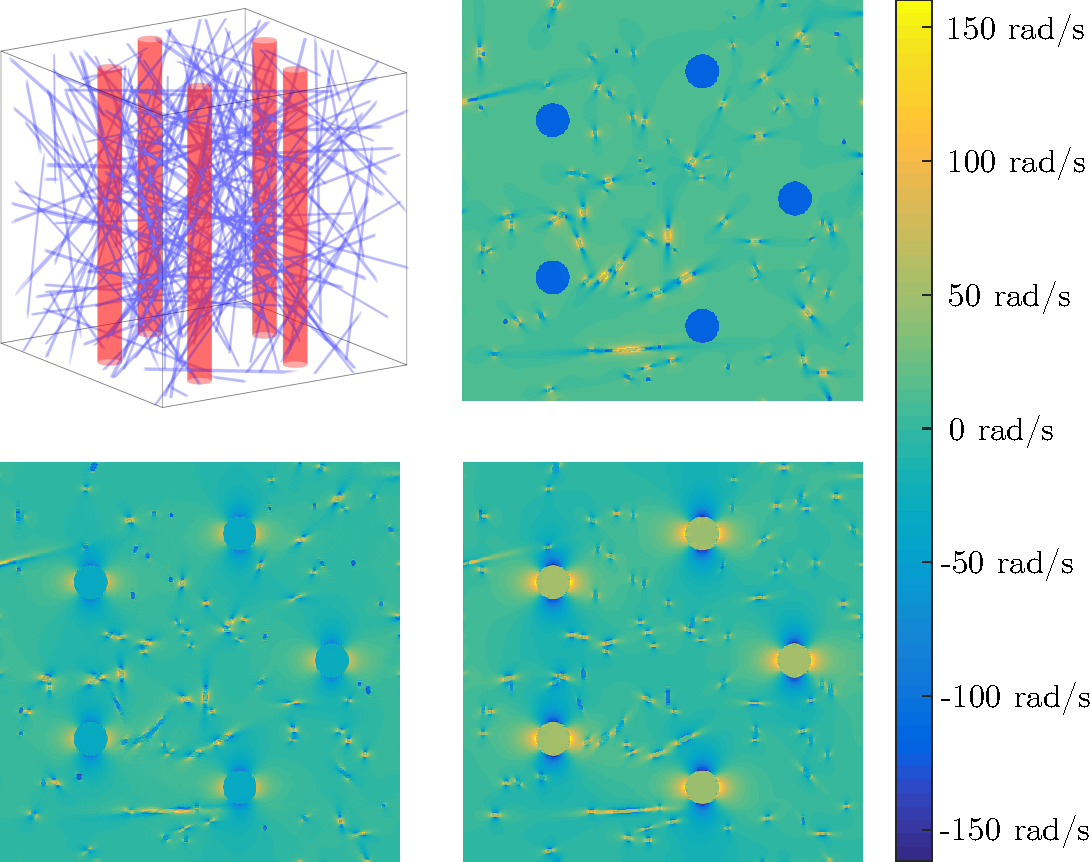
\includegraphics[keepaspectratio=true,width=\textwidth]{spin_echo/voxelgeo_domega_2x2}
    \caption{ The top-left figure shows an example voxel geometry.
      The $3\times 3\times \SI{3}{\milli\meter^3}$
      voxel is populated with an
      isotropic vascular bed and $L=5$ anisotropic large vessels in
      the $z$-direction. The total volume occupied by the blood
      vessels is determined by the blood volume fraction BVF. The
      relative fraction of blood contained in the isotropic vascular
      bed is determined by the isotropic relative blood volume
      fraction iRBVF, and the amount of blood contained in the
      anisotropic vessels is then $\text{aRBVF} = 1 - \text{iRBVF}$.
      The magnetic field generated by this configuration is computed
      by the convolution of the susceptibility map with the unit
      dipole kernel. Example cross-sections of the frequency shift
      map $\delta\omega$ are shown for $\alpha = 0\degree$ (top
      right), $45 \degree$ (bottom left), and $90 \degree$ (bottom
      right).  It can be easily observed that near large vessels, the
      resonance frequency (i.e. the magnetic field) remains locally
      relatively constant compared to the resonance frequency near
      small vessels, which changes rapidly over short distances.  Note
      also the increase in strength and range of inhomogeneities
      around the large anisotropic vessels as $\alpha$ increases,
      introducing the dependence on the angle $\alpha$ into the
      simulations.}
    \label{fig:geometry}
    \end{minipage}
\end{figure}

\clearpage
\begin{figure}[H]
\centering
\begin{minipage}{1.0\textwidth}

\centering
%\begin{minipage}{0.7\textwidth}
\begin{minipage}{1.0\textwidth}
\begin{algorithm}[H]
\setstretch{2.0}
\fontsize{16}{16}
\begin{algorithmic}[1]
    \algsetup{linenosize=\LARGE}
    \algsetup{indent=3em}
    \vspace{0.25cm}
    \STATE \text{\LARGE{}Initialize:} $\Mxy_0 \coloneqq i$,
    $\delta t \coloneqq \text{TE}/30$, $k \coloneqq 0$

    \WHILE{ $k \delta t < \text{TE}$ }
    
    \STATE $\Mxy_{k+\frac{1}{2}} \coloneqq 
    e^{-\CDecay(\v{x}) \delta t} \, \Mxy_k$
    %\COMMENT{$\delta t \rightarrow \delta t/2$}

    \STATE $\Mxy_{k+1} \coloneqq 
    \Phi(\v{x},\delta t) \conv \Mxy_{k+\frac{1}{2}}$
    %\COMMENT{$\Mxy_{k+1} \rightarrow \Mxy_{k+\frac{1}{2}}$}

    %\STATE \Comment{$\Mxy_{k+1} \coloneqq
    %e^{-\CDecay(\v{x}) \delta t/2} \Mxy_{k+\frac{1}{2}}$}

    \IF{ $(k+1) \delta t = \text{TE}/2$ }
    \STATE $\Mxy_{k+1} \coloneqq \conj{\Mxy}_{k+1}$
    \ENDIF
    
    \STATE $k \coloneqq k + 1$
    
    \ENDWHILE
    
    \STATE $S(\text{TE}) \coloneqq \int \Mxy_k \, d^3\v{x}$
\end{algorithmic}
\captionsetup{strut=off}
\caption*{\Large{}\textbf{Magnetization Propagation Algorithm}}
\end{algorithm}
\end{minipage}

%\captionsetup{font=small,skip=0pt}
\addtocounter{figure}{-1} %Want this to be labelled as the first Algorithm
\renewcommand{\figurename}{Algorithm}
\caption{Magnetization propagation algorithm used to simulate the signal
    $S(\text{TE})$ for a given set of free parameters 
    $\text{CA}_{\text{PEAK}}$, BVF, iBVF, and $L$. 
    All four free parameters are encoded solely in the complex decay rate 
    $\CDecay(\v{x})$; the rest of the algorithm does not depend on them.
    The notation $\Mxy_\nu$ is shorthand for 
    $\Mxy(\v{x},\nu \delta t)$ throughout the algorithm.
    If the $\mathcal{O}(\delta t^3)$ order evolution 
    equation~\eqref{EvolSplit_Order3} were used instead,
    line 3 should be modified to decay for only a half time step $\delta t/2$,
    line 4 should perform the Gaussian convolution in-place,
    and an extra line should be added directly following the convolution which
    decays for another half time step $\delta t/2$.}
    \label{fig:algorithm1}
\end{minipage}
\end{figure}

\clearpage
\begin{figure}[H]
\centering
\begin{minipage}{1.0\textwidth}
    \centering
    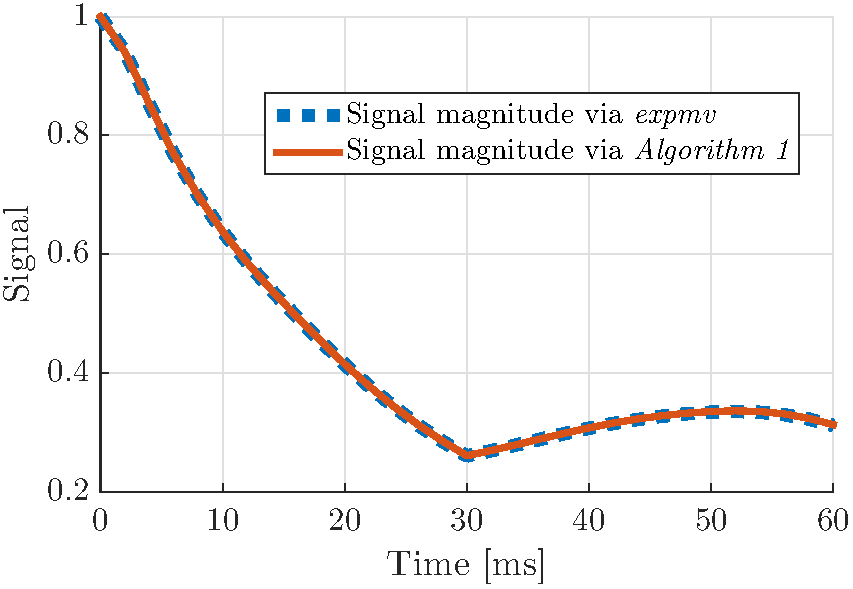
\includegraphics[keepaspectratio=true,width=1.0\textwidth]{spin_echo/SE_Signal_vs_Time_ConvDiff_vs_Expmv}
    \caption{Comparison between solving the Bloch-Torrey equation exactly using the method of lines in conjunction with Higham's \textit{expmv} integrator~\cite{al-mohy_computing_2011}, and solving the Bloch-Torrey equation approximately using the two-step approximate solution as described in Algorithm~\ref{fig:algorithm1}.
    The signal decay through time calculation shows strong agreement between the two methods, with error values of 0.064\% +/- 0.045\%; the maximum error value of 0.14\% occurs at $\unit[60]{ms}$.}
    \label{fig:comparison}
\end{minipage}
\end{figure}

\end{document}
